\capitulo{6}{Trabajos relacionados}

En este capítulo revisamos el trabajo previo en el campo de estudio de análisis inmobiliario mediante Aprendizaje Automático y como ha afectado al desarrollo del proyecto.

De forma significativa, encontramos un artículo de Baldominos et al.~\cite{baldominos2018} que destaca la utilización de métodos variados de \textit{Machine Learning}, incluyendo conjuntos de árboles de regresión, regresión de vectores de soporte, \textit{k-nearest neighbors} y redes neuronales. Pese a la diversidad de enfoques, en el artículo se resalta una notable escasez de investigaciones que apliquen directamente el \textit{Machine Learning} en la valoración de propiedades inmobiliarias. El documento propone un innovador enfoque de regresión utilizando características extraídas de listados en línea para estimar precios de mercado, marcando un punto de partida significativo para futuros estudios y además, el presente proyecto. 

El estudio de Niu et al.~\cite{niu2019} introduce un sistema de valoración inmobiliaria avanzado que aprovecha técnicas de \textit{Machine Learning} no solo para evaluar los inmuebles sino también para abordar desafíos específicos como la identificación de registros duplicados y la extracción/identificación efectiva de características a usar en los modelos. La identificación de registros duplicados resulta esencial si se extraen datos de distintos portales inmobiliarios, ya que los anuncios habitualmente están repetidos. Además, el enfoque del artículo, resalta la importancia de aplicar un conjunto de múltiples modelos a la vez, como \textit{Gradient Boosting Decission Trees}, \textit{Random Forest} y redes neuronales de tipo \textit{Back Propagation} (BP), para mejorar la precisión en la valoración de propiedades. Los resultados experimentales obtenidos con datos de propiedades en Hangzhou, China, demuestran la superioridad de su sistema combinado, suponiendo un interesante punto de partida para la posible futura expansión del actual proyecto.

Otro punto interesante, volviendo al artículo de Baldominos et al.~\cite{baldominos2018}, es que en este se estudia un solo barrio, el barrio de Salamanca de Madrid. Se muestra cómo este enfoque, barrio por barrio, es más potente, ya que en cada zona de una ciudad se crea un mercado diferenciado y se valoran distintas características de los inmuebles. Dentro de la misma ciudad, Madrid, es muy distinto el barrio de Salamanca al de Carabanchel. También debemos señalar, que este modelo barrio por barrio hace mucho más difícil escalar el proyecto a nivel de todo un país, sobre todo por la falta de suficientes datos. En ciudades pequeñas o medianas, es habitual que solo haya algunos inmuebles a la venta en un determinado barrio en un determinado período de tiempo, siendo insuficientes para entrenar un modelo. También es cierto, que en ciudades pequeñas o medianas suele haber menos heterogeneidad entre barrios. Sería interesante, para futuros estudios, la intersección entre un mecanismo híbrido, donde en provincias o ciudades con suficientes datos, se aplican modelos a nivel de barrio y en zonas con insuficientes datos, se aplique a nivel provincial o municipal.

Finalmente, en el artículo se observa que los modelos que mejores resultados obtienen son los árboles de regresión conjuntos, o \textit{Ensembles of Regression Trees} (Figura \ref{fig:model_results_baldominos}). Esto resulta consistente con lo observado en el presente proyecto, donde en la mayoría de las provincias el modelo con mejor resultado suele ser un árbol de regresión conjunto. 

\begin{figure}[ht]
    \centering
    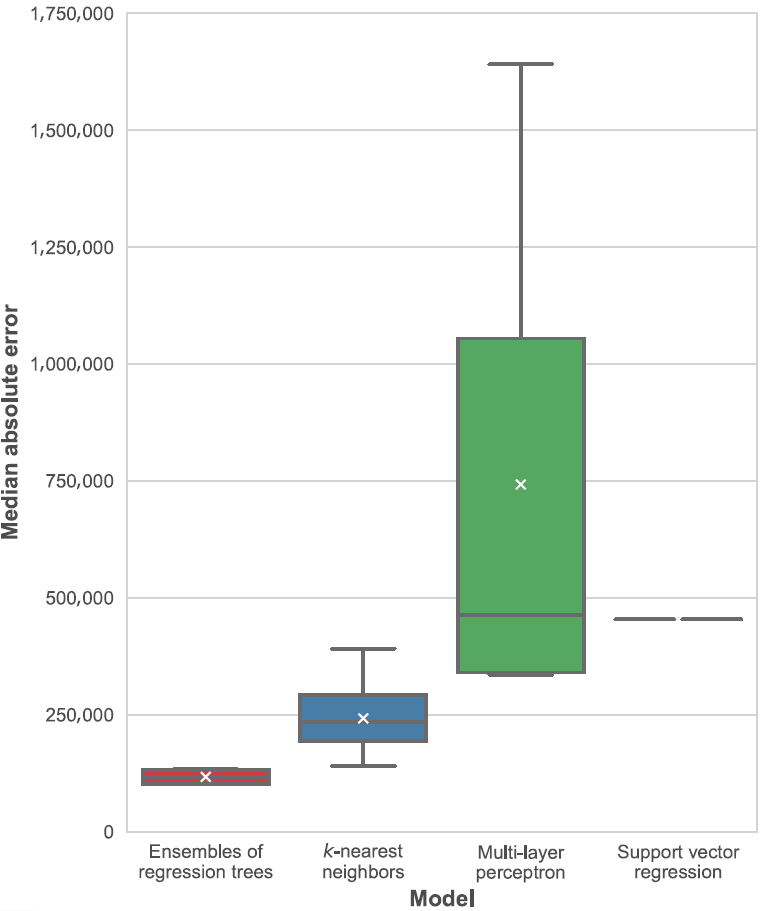
\includegraphics[width=0.8\textwidth]{img/Figura9.PNG}
    \caption[Resultados de MAE (Median Absolute Error) de los distintos tipos de modelos para regresión de precios en Barrio de Salamanca, Madrid]{Resultados de MAE (\textit{Median Absolute Error}) de los distintos tipos de modelos para regresión de precios en Barrio de Salamanca, Madrid~\cite{baldominos2018}. En el eje $Y$, vemos MAE en € y en el eje $X$ los distintos tipos de modelos analizados.}
    \label{fig:model_results_baldominos}
\end{figure}


En el presente proyecto se han separado los modelos de \textit{Machine Learning} a nivel de provincia, construyendo así dos modelos por provincia, uno para inmuebles ``caros'' y otro para inmuebles ``baratos'' (Para detalles ver Sección \ref{sec:provincias}). Los modelos no van a ser tan precisos como los utilizados en el enfoque que se hizo en~\cite{baldominos2018},  sin embargo, permiten escalar el proyecto a nivel de estudio inmobiliario de todo un país, habiendo pocos precedentes similares en la literatura.



